% !TeX root = RJwrapper.tex
\title{Current status and propsects of R-packages for the design of
experiments}
\author{by Emi Tanaka}

\maketitle

\abstract{%
Re-running an experiment is generally costly and in some cases
impossible due to limited resources, so the design of experiment plays a
critical role in increasing the quality of experimental data. In this
article I describe the current state of the R-packages for the design of
experiments through textual analysis and download trends. I discuss also
the software design of widely utilised R packages in the field of
experimental design and conclude with discussion of some future
prospects for the field.
}

\hypertarget{introduction}{%
\section{Introduction}\label{introduction}}

The critical role of data collection is well captured in the expression
``garbage in, garbage out'' -- in other words, if the collected data is
rubbish then no analysis, however complex it may be, can make something
out of it. Methods for data collection can be dichotomised by the type
of data collected -- namely, experimental or observational -- or
alternatively, categorised as experimental design (including
quasi-experimental design) or survey design. This dichotomisation, to a
great extent, is seen in CRAN task views where R-packages in
experimental design are in \ctv{ExperimentalDesign} and R-packages in
survey designs are in \ctv{OfficialStatistics}. Survey designs often,
although not always, aim to collect observational data whilst
experimental designs exclusively center on experimental data. This paper
is concerned with the latter.

In the CRAN task view of \ctv{ExperimentalDesign}, there are 107 R
packages for experimental design and analysis of data from experiments,
henceforth referred to as ``DoE packages'' in this paper. The sheer
quantity and variation in the output experimental design in the
R-packages are arguably unmatched with any other programming languages,
e.g.~in Python \citep{python}, only a handful of libraries that generate
design of experiment exist (namely \texttt{pyDOE}, \texttt{pyDOE2},
\texttt{dexpy}, \texttt{experimenter} and \texttt{GPdoemd}) with limited
outputs. Thus, the study of DoE packages is also revealing into the
current status of the field of experimental design.

The paper is organisd as follows. Section @ref(eda)

\hypertarget{eda}{%
\section{Explorative analysis}\label{eda}}

\begin{Schunk}
\begin{figure}[htbp]

{\centering 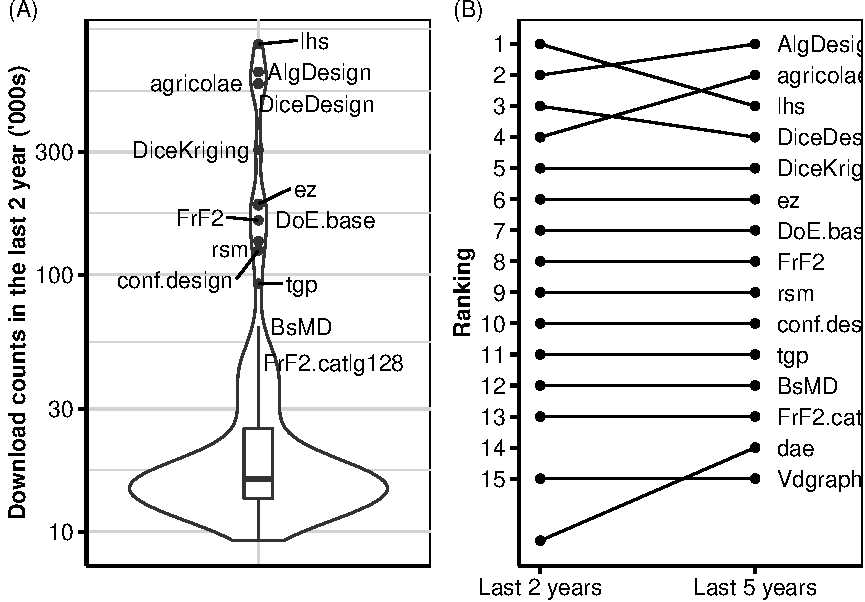
\includegraphics{figures/dlplots-1} 

}

\caption[The above graph shows the total download counts from 2020-03-10 to 2022-03-08 of DoE packages]{The above graph shows the total download counts from 2020-03-10 to 2022-03-08 of DoE packages.}\label{fig:dlplots}
\end{figure}
\end{Schunk}

\begin{itemize}
\tightlist
\item
  Not much difference between title and description.
\item
  Just go with description and combine bi \& tri.
\end{itemize}

\begin{Schunk}


\begin{center}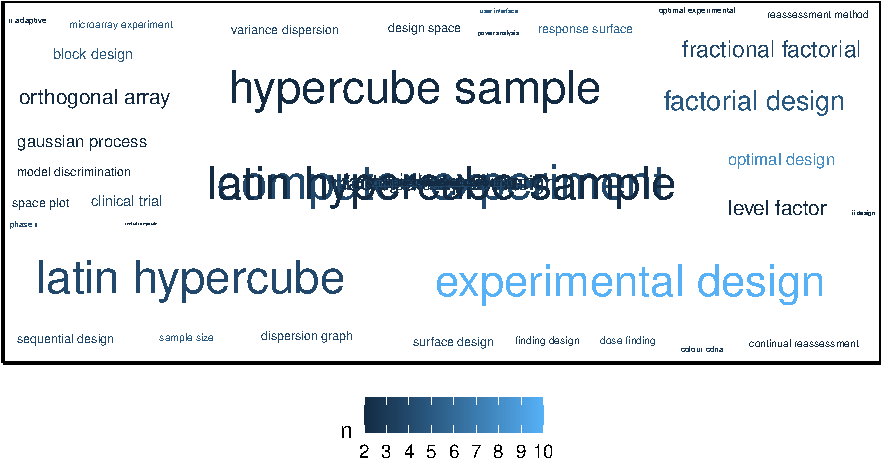
\includegraphics{figures/wordcloud-1} \end{center}

\end{Schunk}

\hypertarget{what-are-the-common-types-of-experimental-designs}{%
\subsection{What are the common types of experimental
designs?}\label{what-are-the-common-types-of-experimental-designs}}

\hypertarget{how-do-packages-interplay-with-each-other}{%
\subsection{How do packages interplay with each
other?}\label{how-do-packages-interplay-with-each-other}}

\hypertarget{which-packages-are-widely-utilised}{%
\subsection{Which packages are widely
utilised?}\label{which-packages-are-widely-utilised}}

Figure \ref{fig:dlplots} suggests that the \CRANpkg{AlgDesign} followed
by \CRANpkg{agricolae} are far more downloaded than any other DoE
packages. It is worth noting that \CRANpkg{agricolae} imports
\CRANpkg{AlgDesign} thus any download of \CRANpkg{agricolae} likely
results also in a download of \CRANpkg{AlgDesign}.

\hypertarget{software-design}{%
\section{Software design}\label{software-design}}

\hypertarget{discussion}{%
\section{Discussion}\label{discussion}}

An experiment involves running a number of steps:

\begin{enumerate}
\def\labelenumi{\arabic{enumi}.}
\tightlist
\item
  Defining the hypothesis or question
\item
  Formulating methods to test hypothesis or answer question
\item
  Planning the experimental protocol:
\end{enumerate}

\begin{itemize}
\tightlist
\item
  Determining experimental resources,
\item
  specifying the data collection procedure,
\item
  constructing the experimental design layout, and
\item
  proposing a model for analysis.
\end{itemize}

\begin{enumerate}
\def\labelenumi{\arabic{enumi}.}
\setcounter{enumi}{3}
\tightlist
\item
  Collect data
\item
  Analyse data, interpret result and conclusion
\end{enumerate}

\newpage

\begin{table}[h] \centering  
\begin{tabular}[t]{lr}
\toprule
word & n\\
\midrule
experimental design & 8\\
optimal design & 7\\
clinical trial & 5\\
dose finding & 5\\
block design & 4\\
microarray experiment & 4\\
response surface & 4\\
sequential design & 4\\
\bottomrule
\end{tabular} \hspace{1cm} \centering  
\begin{tabular}[t]{lr}
\toprule
word & n\\
\midrule
experimental design & 10\\
optimal design & 8\\
response surface & 6\\
block design & 5\\
contour plot & 5\\
effect model & 5\\
factorial design & 5\\
graphical user & 5\\
microarray experiment & 5\\
mixed effect & 5\\
package provide & 5\\
sample size & 5\\
user interface & 5\\
\bottomrule
\end{tabular} \caption{My tables} \end{table}

\bibliography{../paper.bib}

\address{%
Emi Tanaka\\
Monash University\\%
Monash University\\ Clayton campus, VIC 3800, Australia\\
%
\url{http://emitanaka.org/}\\%
\textit{ORCiD: \href{https://orcid.org/0000-0002-1455-259X}{0000-0002-1455-259X}}\\%
\href{mailto:emi.tanaka@monash.edu}{\nolinkurl{emi.tanaka@monash.edu}}%
}
